\documentclass{article}
\usepackage[utf8]{inputenc}
\usepackage{graphicx}
\usepackage{float}
\usepackage{hyperref}


\title{RH PWR guardian (manual)}
\author{Daniel Vander-Hyde, Stefan Ballmer, Thomas Vo, TJ Shaffer}
\href{mailto:dcvander@syr.edu}{dcvander@syr.edu}
\date{February 2019}

\begin{document}

\maketitle

\section{Introduction}
We measured the input ring heater (RH) power to test mass (TM) spherical power transfer function of the ALIGO input test masses (ITM) and end test masses (ETM) and discovered that the time it takes to be within 10\% of the nominal thermal lens is about $\approx 10.88$ hours. We propose a strategy that uses an inverted digital plant filter to condition the input power requests to reduce this time to ~1.54 hours. The plant here being the ring heater / test mass system. We split the next section into three different sub-sections. Sections 2.1 and 2.2 mostly apply to the general usage of the TCS\_(OPTIC)\_RH\_PWR guardians, while Section 2.3 details what is occurring in these guardian states. This document assumes you already have a digital inverse plant filter in \$(IFO)TCSCS\_ \$(OPTIC)\_RH\_INVERSE\_FILTER. If you do not, please take the time to measure the step response and consult the supplementary ipython notebook for performing the digital plant filter inversion. 

\section{Using the TCS\_RH\_PWR Guardian}
The intention of this guardian is to allow the user to have more control of the filtering process of the RH power input. Using the guardian state machine architecture, we split up this guardian into 3 different states: NOMINAL, FILTER\_RH\_INPUT, and RESET. The essential filters, channels and inner workings of these states live within the TCS simulink model. The filters that are composed within this model are: An inverse plant filter (which we call the inverse ring heater filter), the inverse of the inverse plant filter (which one might think would be identical to the plant filter but isn't quite because of the additional tuning of inverse filters for stability.

\subsection{Making a filtered change in RH power}
Before making a change in power you might want to check that the "Filter input" value matches that of the requested power of the corresponding TM. If it is not, you will want to first go to the RESET state first to set the filter input offset equal to the current power.  
To make a change in RH power with the inverse filter, one needs to change the guardian to the FILTER\_RH\_INPUT state. This will then allow you to change the "Filter input" any number amount of times and the filter should modify the power so the convergence to the nominal lens will occur within 3 hours. From whatever last change you have made, you will want to leave the filter running for the next two days to maintain the lens change, then you can switch back to nominal if you'd like

\subsection{Making an unfiltered change in RH power}
You will want to be in the NOMINAL state when making this change. After making the change, it is suggested that you update the input filter offset by going to RESET and back to NOMINAL so that the FILTER\_RH\_INPUT state can operate when you do request to make a filtered change. 

\subsection{Going back on a filtered change}
In the case you are making a filtered change and you want change the output back to the original output power, you have the option of going from the FILTER\_RH\_INPUT state, to the RESET state, to NOMINAL. From there, you can change the power back to the original value and set your $\mu$ back to the original value by gong to RESET and back to NOMINAL.

\subsection{Guardian States}
\subsubsection{NOMINAL}
\begin{figure}[H]
    \centering
    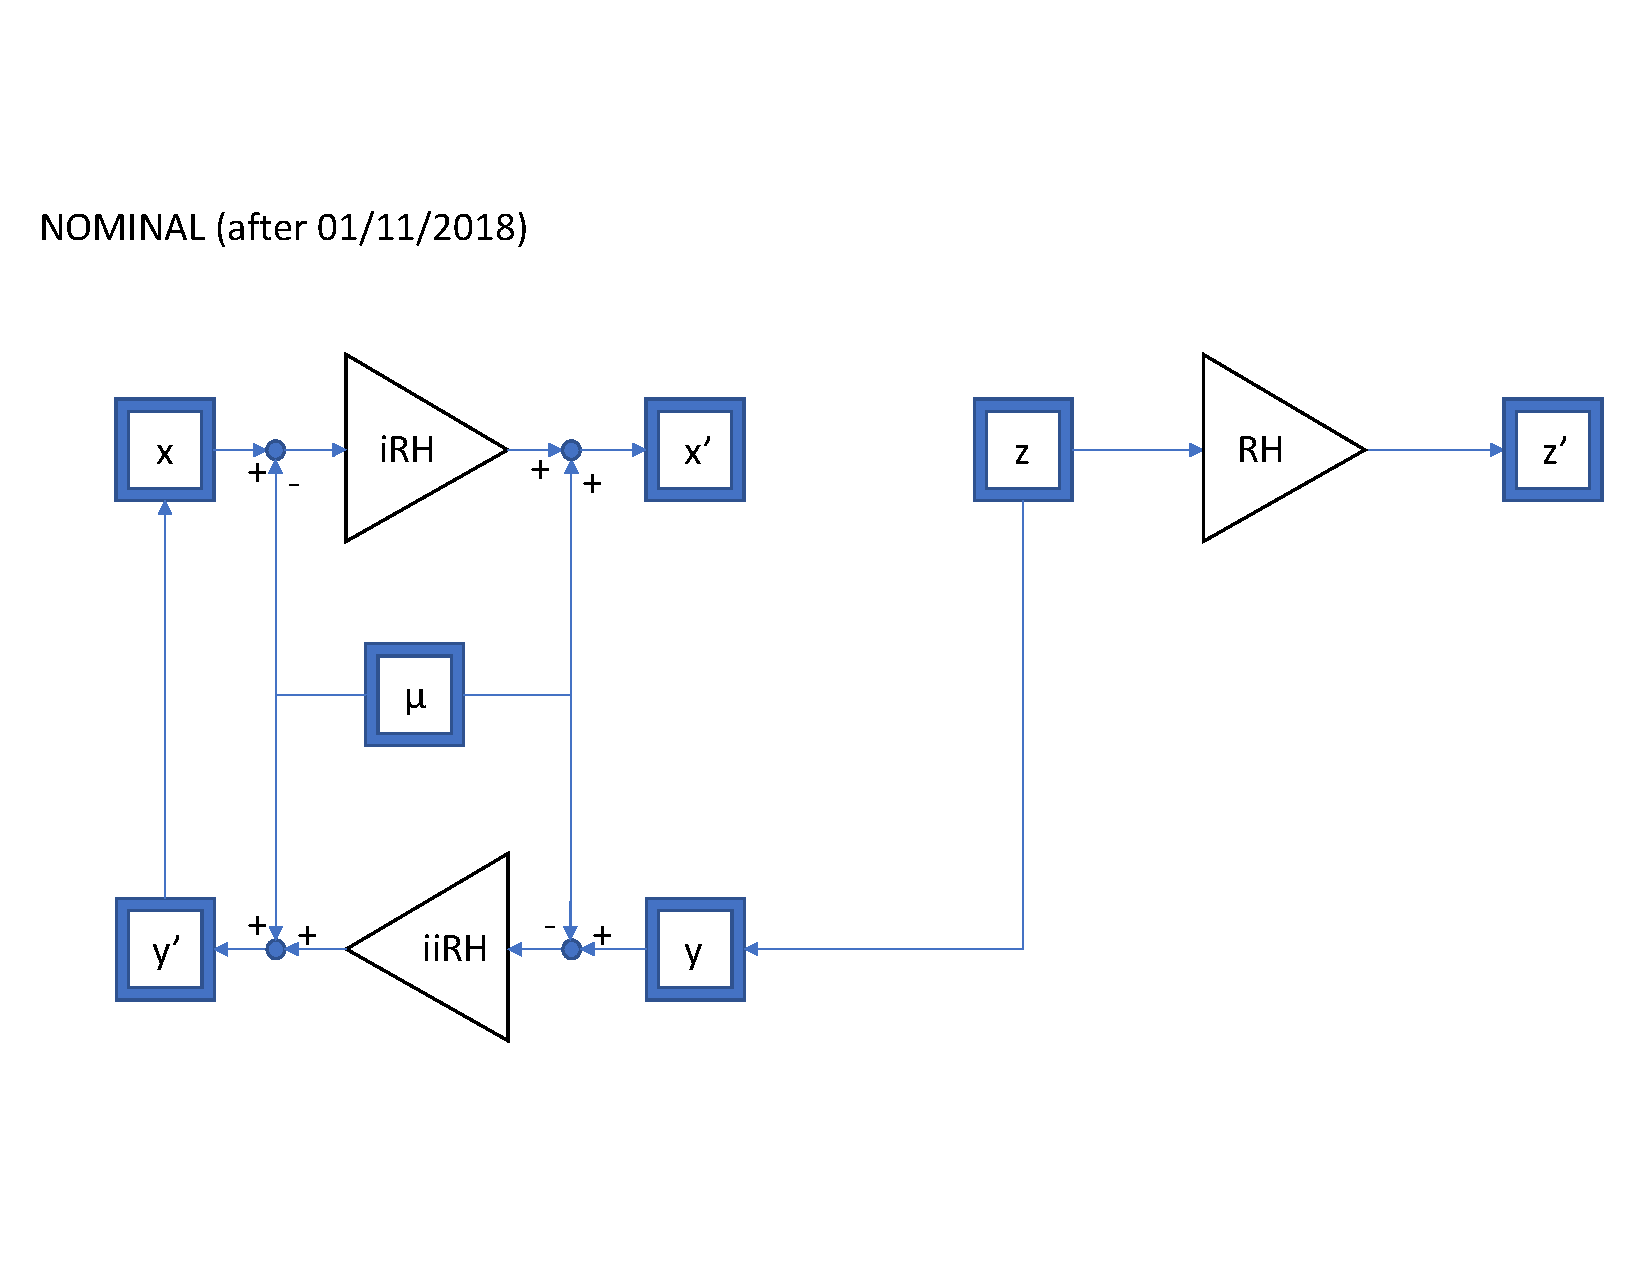
\includegraphics[width=1\textwidth]{NOMINAL_DIAGRAM.pdf}
    \caption{A controls diagram of the NOMINAL guardian state. Essential connections unique to this state are the y' -> x connection which essentially wires the output of the iiRH (inverse inverse plant filter), to the the input of the iRH (inverse plant filter)}
\end{figure}

\begin{itemize}
\item This state is to be the state the guardian will be in when: 
\subitem No power changes are made
\subitem The user wants to make an unfiltered power change
\end{itemize}

\subsubsection{FILTER\_RH\_POWER}

%\begin{itemize}
%\end{itemize}

\begin{figure}[H]
    \centering
    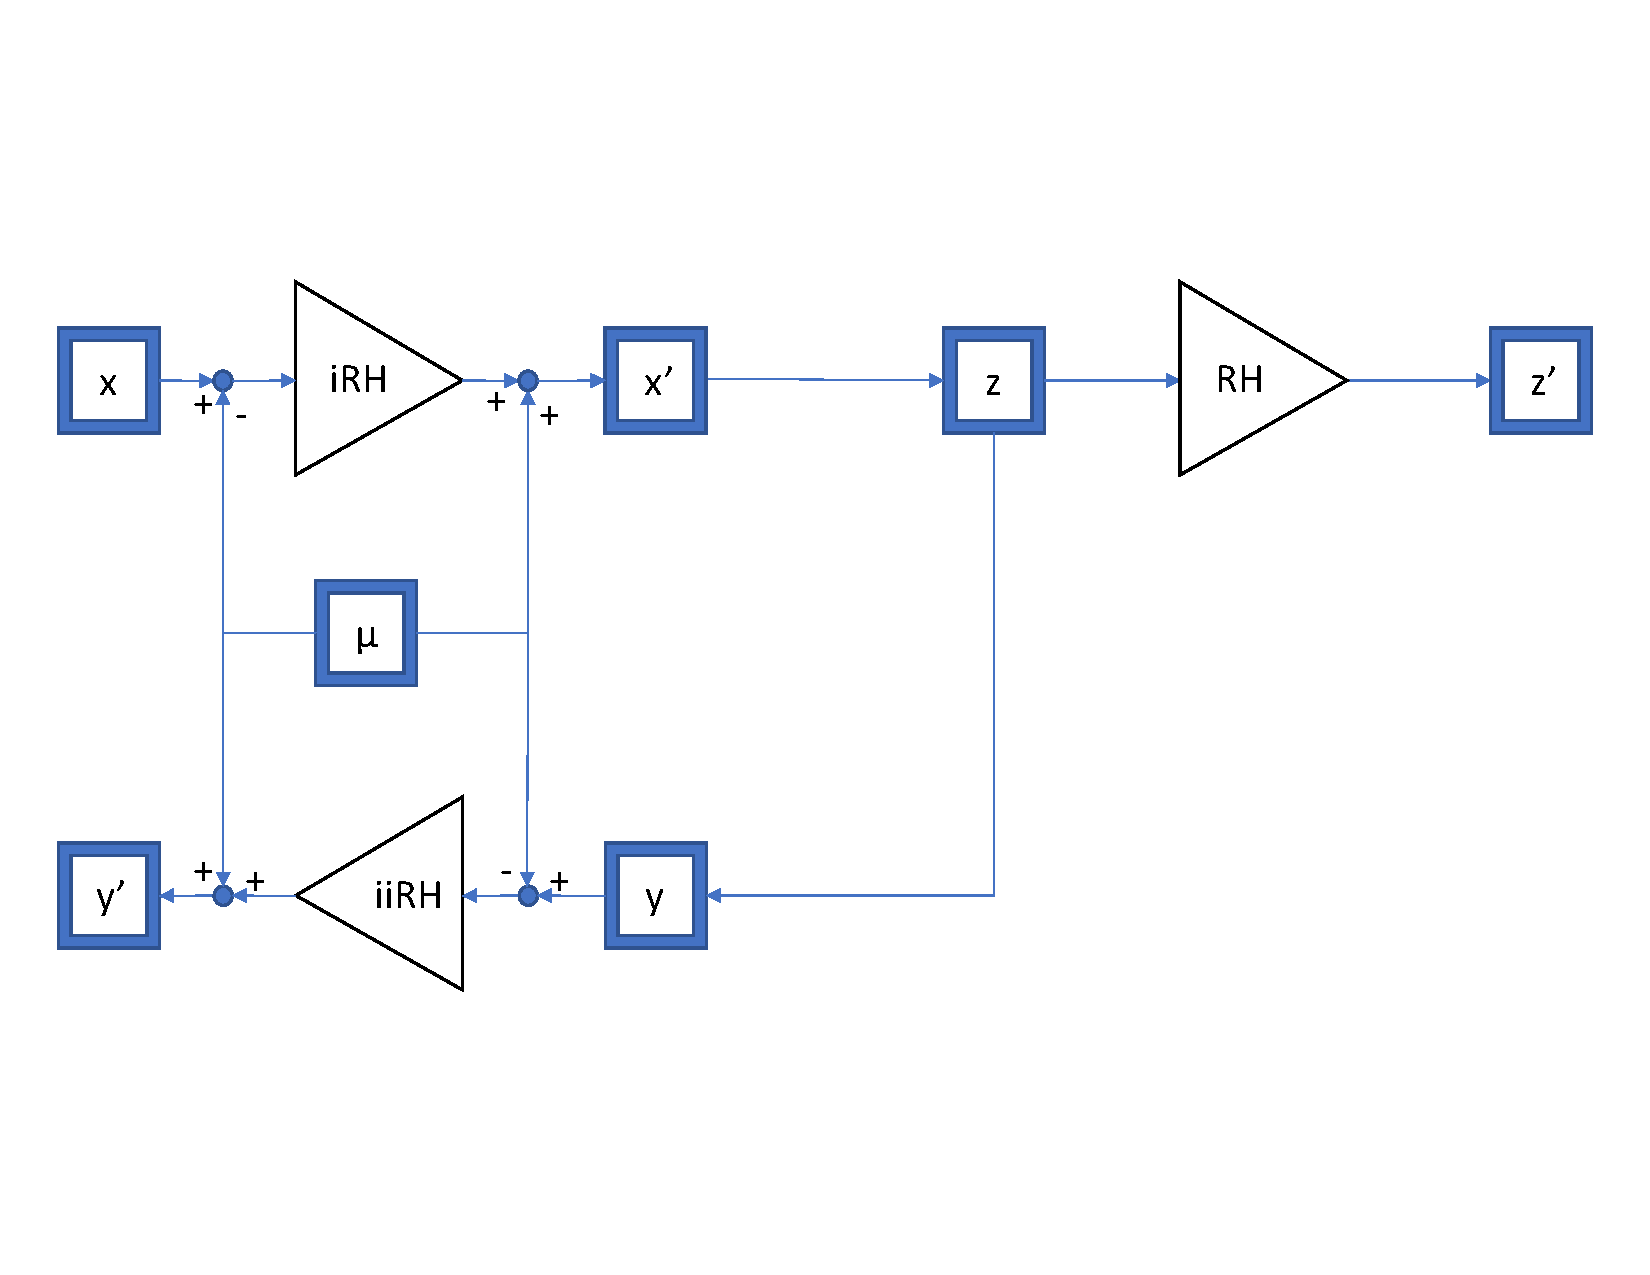
\includegraphics[width=1\textwidth]{FILTER_RH_INPUT_DIAGRAM.pdf}
    \caption{A controls diagram of the FILTER\_RH\_INPUT state. The connection unique to this state is between x' and z. This sets the output of the iRH to the input of the plant. }
\end{figure}
\subsubsection{RESET}
\begin{itemize}
\item From NOMINAL
	\subitem If you are transitioning from the NOMINAL state to the reset state, you will:
		\subsubitem Update your reset $\mu$ (Filter DC offset) value 
		\subsubitem Clear the history on iRH and iiRH
\subitem

\item From FILTER\_RH\_INPUT
	\subitem If you are transitioning from the FILTER\_RH\_INPUT state, you will: 
		\subsubitem Update your $\mu$ value (Filter DC offset) with the input from of iRH (be aware that if entered into prematurely, this sets $\mu$ to the final value the filter would have reached if the filter was untouched)
		\subsubitem Clear the history on iRH and iiRH
\end{itemize}

\end{document}

